\documentclass{beamer}
\usetheme{Madrid}
\usepackage{multicol}
\usepackage{longtable}
\title{Global Remittance System}
\author{Presented by: Philip Mensah \& Jorge Alvarez}
\institute{UNLV}
\date{\today}



\begin{document}

\begin{frame}
  \titlepage
\end{frame}

% The rest of the presentation follows...


\begin{frame}{Background}
    \begin{itemize}
        \item What is a Remittance? Who are the players?
        \item What is the process?
        \item Is there room for additional players in the market?
    \end{itemize}
    
\end{frame}



\begin{frame}{Functions}
    \begin{multicols}{2}
        \begin{itemize}
            \item User Registration
    \item Update User
    \item User Login
    \item Transaction History
    \item Create Remittance
    \item Calculate Fees
    \item Currency Converter
        \end{itemize}
    \columnbreak
    \begin{itemize}
        \item Process Remittance
    \item Cancel Remittance
    \item Receive Remittance
    \item Update Exchange Rates
    \item Partner Settle
    \item Send Notification
    \end{itemize}
    \end{multicols}
    
\end{frame}

\begin{frame}{Login Screen}
    \begin{figure}
        \centering
        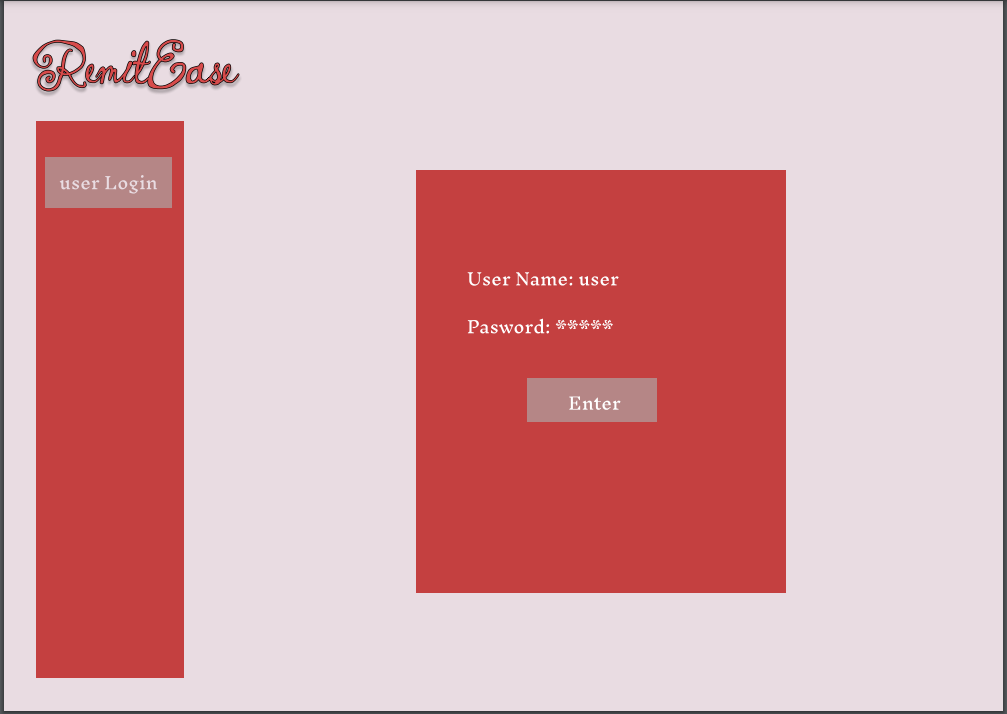
\includegraphics[width=.7\linewidth]{MockUps/login.PNG}
        \caption{A mockup of a login screen for an application named "RemitEase." The mockup presents a simple and user-friendly interface with the log in form.}
        \label{fig:enter-label}
    \end{figure}
\end{frame}

\begin{frame}{Main Screen with System Functions}
    \begin{figure}
        \centering
        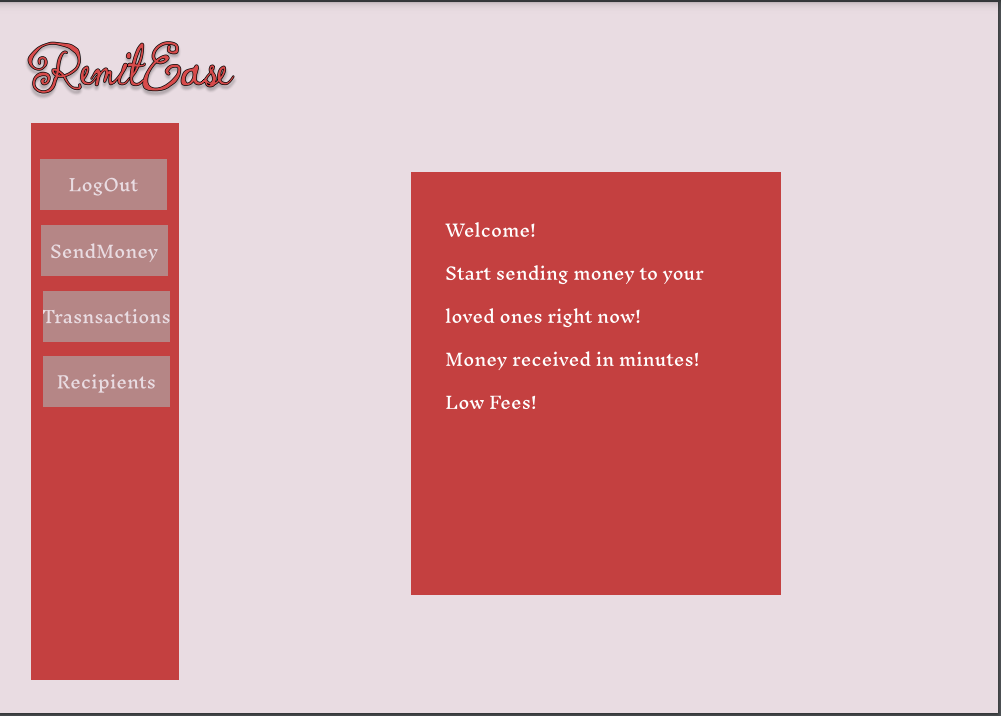
\includegraphics[width=.7\linewidth]{MockUps/2welcome.PNG}
        \caption{Main screen with a navigation sidebar pointing to system functions.}
        \label{fig:enter-label}
    \end{figure}
\end{frame}

\begin{frame}{Add New Recipient or Use Existing Recipient}
    \begin{figure}
        \centering
        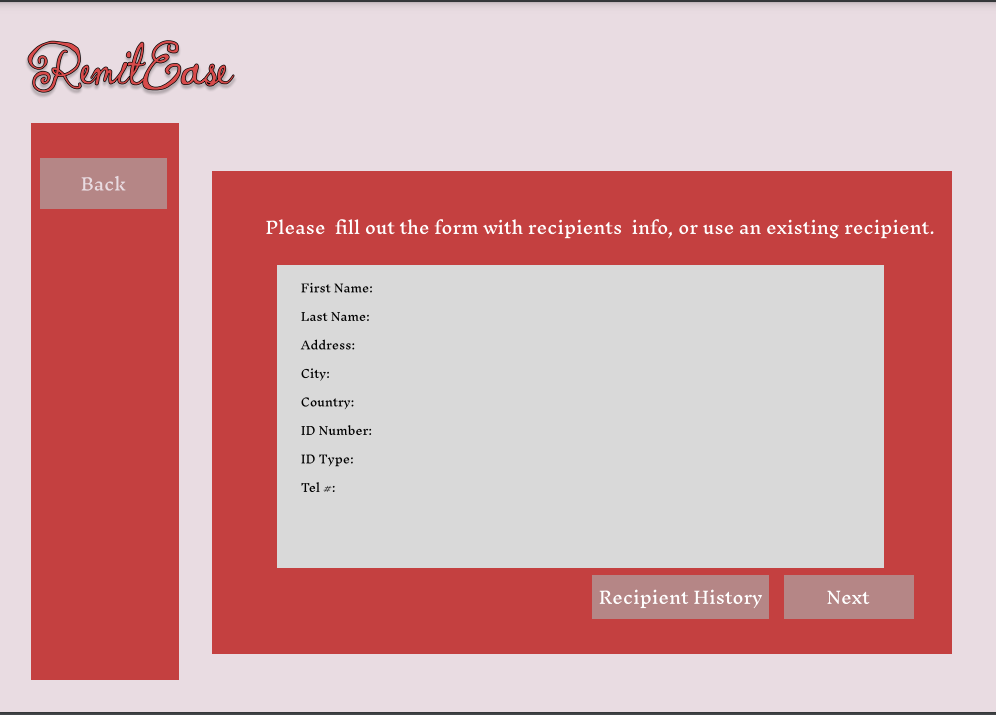
\includegraphics[width=.7\linewidth]{MockUps/3ReceipientsInfoForm.PNG}
        \caption{Customer that initiates a new remittance has the function to add a new recipient.}
        \label{fig:enter-label}
    \end{figure}
\end{frame}

\begin{frame}{Add Amount}
    \begin{figure}
        \centering
        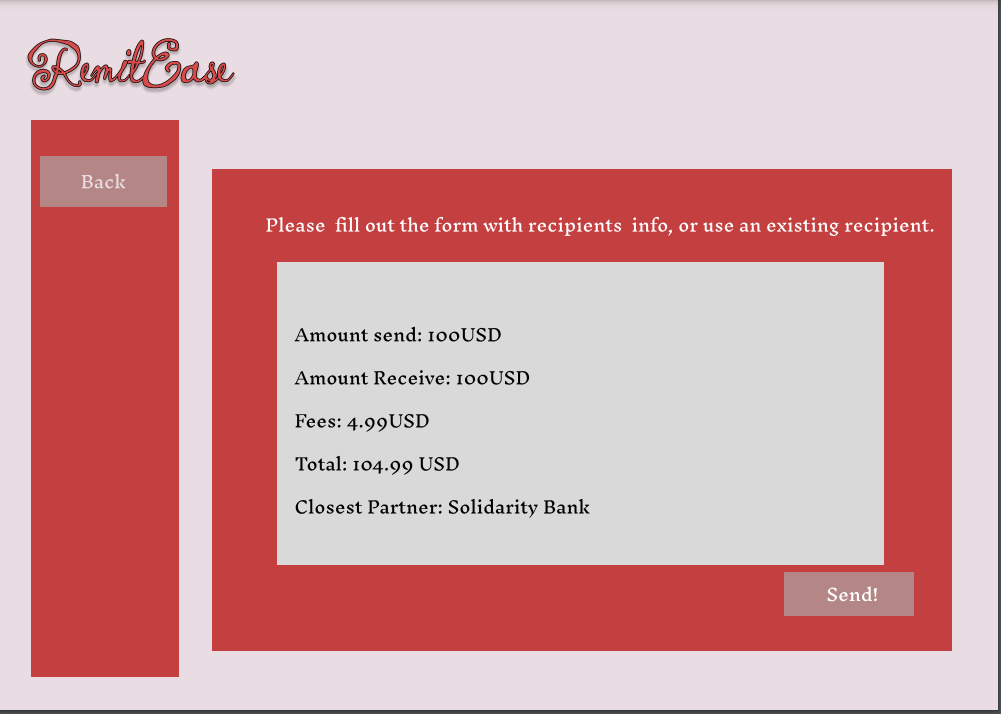
\includegraphics[width=.7\linewidth]{MockUps/AmountScreen.PNG}
        \caption{After recipient details are added, the program offers the function to input remittance amount. Then it shows receive amount in target currency and fees as a function of remittance amount.}
        \label{fig:enter-label}
    \end{figure}
\end{frame}

\begin{frame}{List of Recipients}
    \begin{figure}
        \centering
        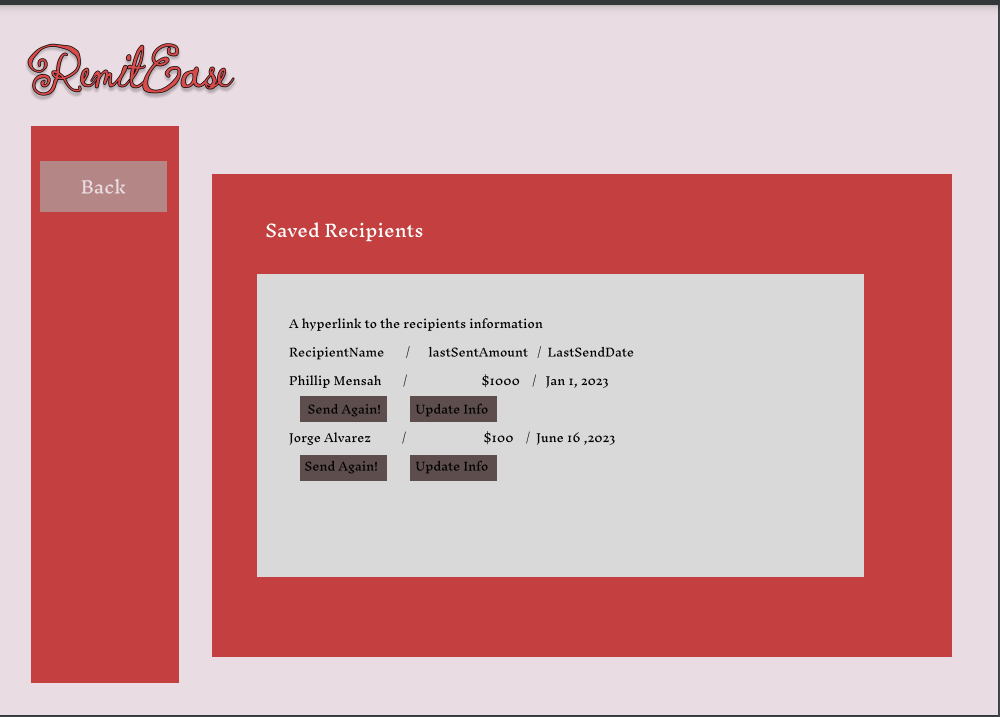
\includegraphics[width=.7\linewidth]{MockUps/Recipients.PNG}
        \caption{Function that shows the list of saved recipients and a function to send remittance or update/delete the saved recipient.}
        \label{fig:enter-label}
    \end{figure}
\end{frame}

\begin{frame}{Confirmation For Adding A Recipient}
    \begin{figure}
        \centering
        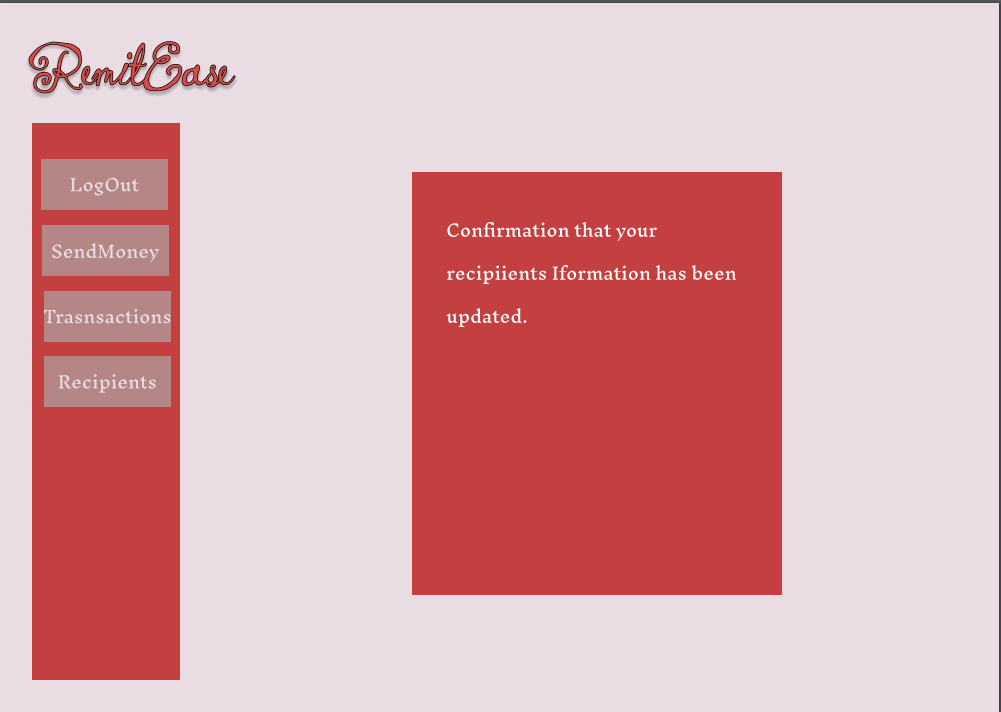
\includegraphics[width=.7\linewidth]{MockUps/RecipientUpdateConfirmation.PNG}
        \caption{Backend function has updated the recipient details. Front end shows confirmation.}
        \label{fig:enter-label}
    \end{figure}
\end{frame}

\begin{frame}{Notification}
    \begin{figure}
        \centering
        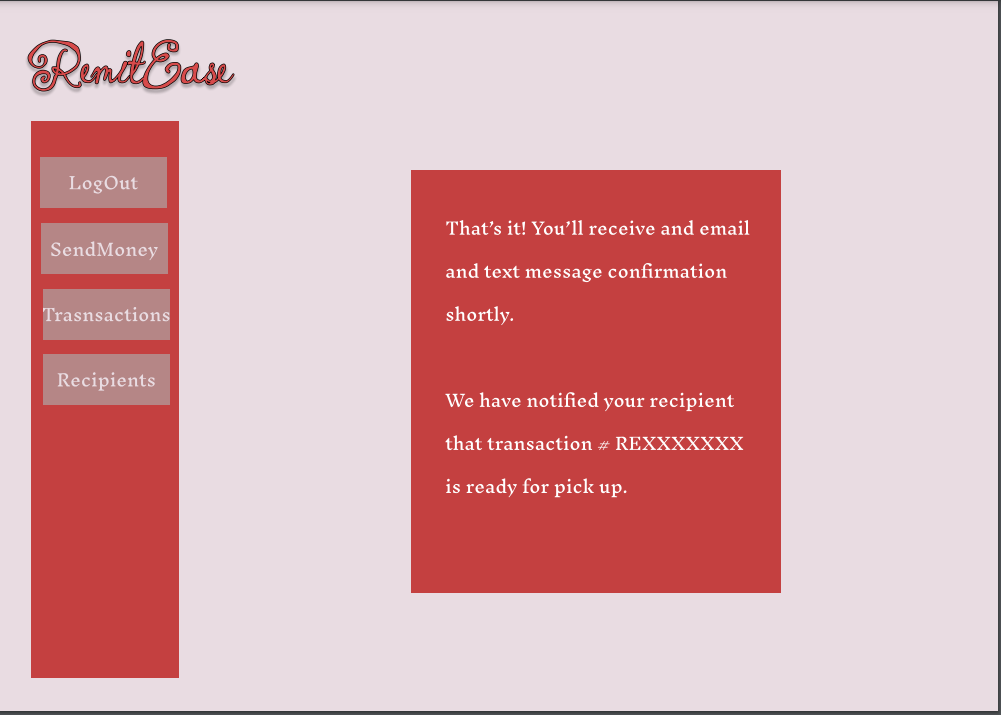
\includegraphics[width=.7\linewidth]{MockUps/SendConfirmation.PNG}
        \caption{Backend function has processed the transaction. Front end function shows the confirmation.}
        \label{fig:enter-label}
    \end{figure}
\end{frame}

\begin{frame}{Transaction History and Status}
    \begin{figure}
        \centering
        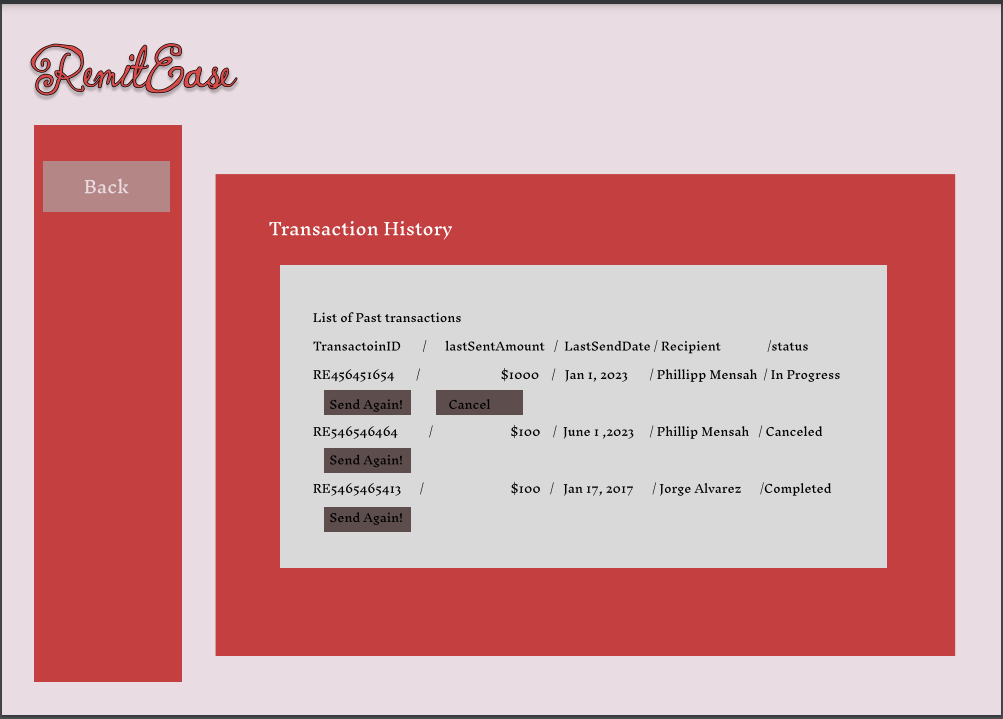
\includegraphics[width=.7\linewidth]{MockUps/TransactionHist.PNG}
        \caption{Function to show transaction history and status. Function to send again. Function to cancel pending transaction.}
        \label{fig:enter-label}
    \end{figure}
\end{frame}


\begin{frame}{Notification for a Cancelled Transaction}
    \begin{figure}
        \centering
        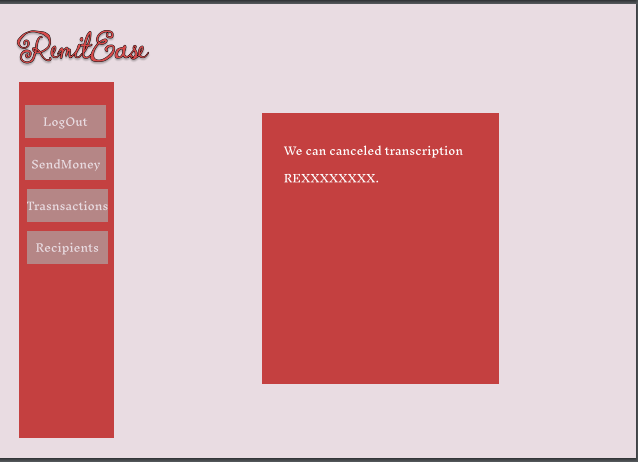
\includegraphics[width=.7\linewidth]{MockUps/CancelConfirmation.PNG}
        \caption{Backend has successfully changed the status of the transaction  to cancelled. Front end shows confirmation.}
        \label{fig:enter-label}
    \end{figure}
\end{frame}


\begin{frame}{Class Diagram}
\begin{figure}
    \centering
    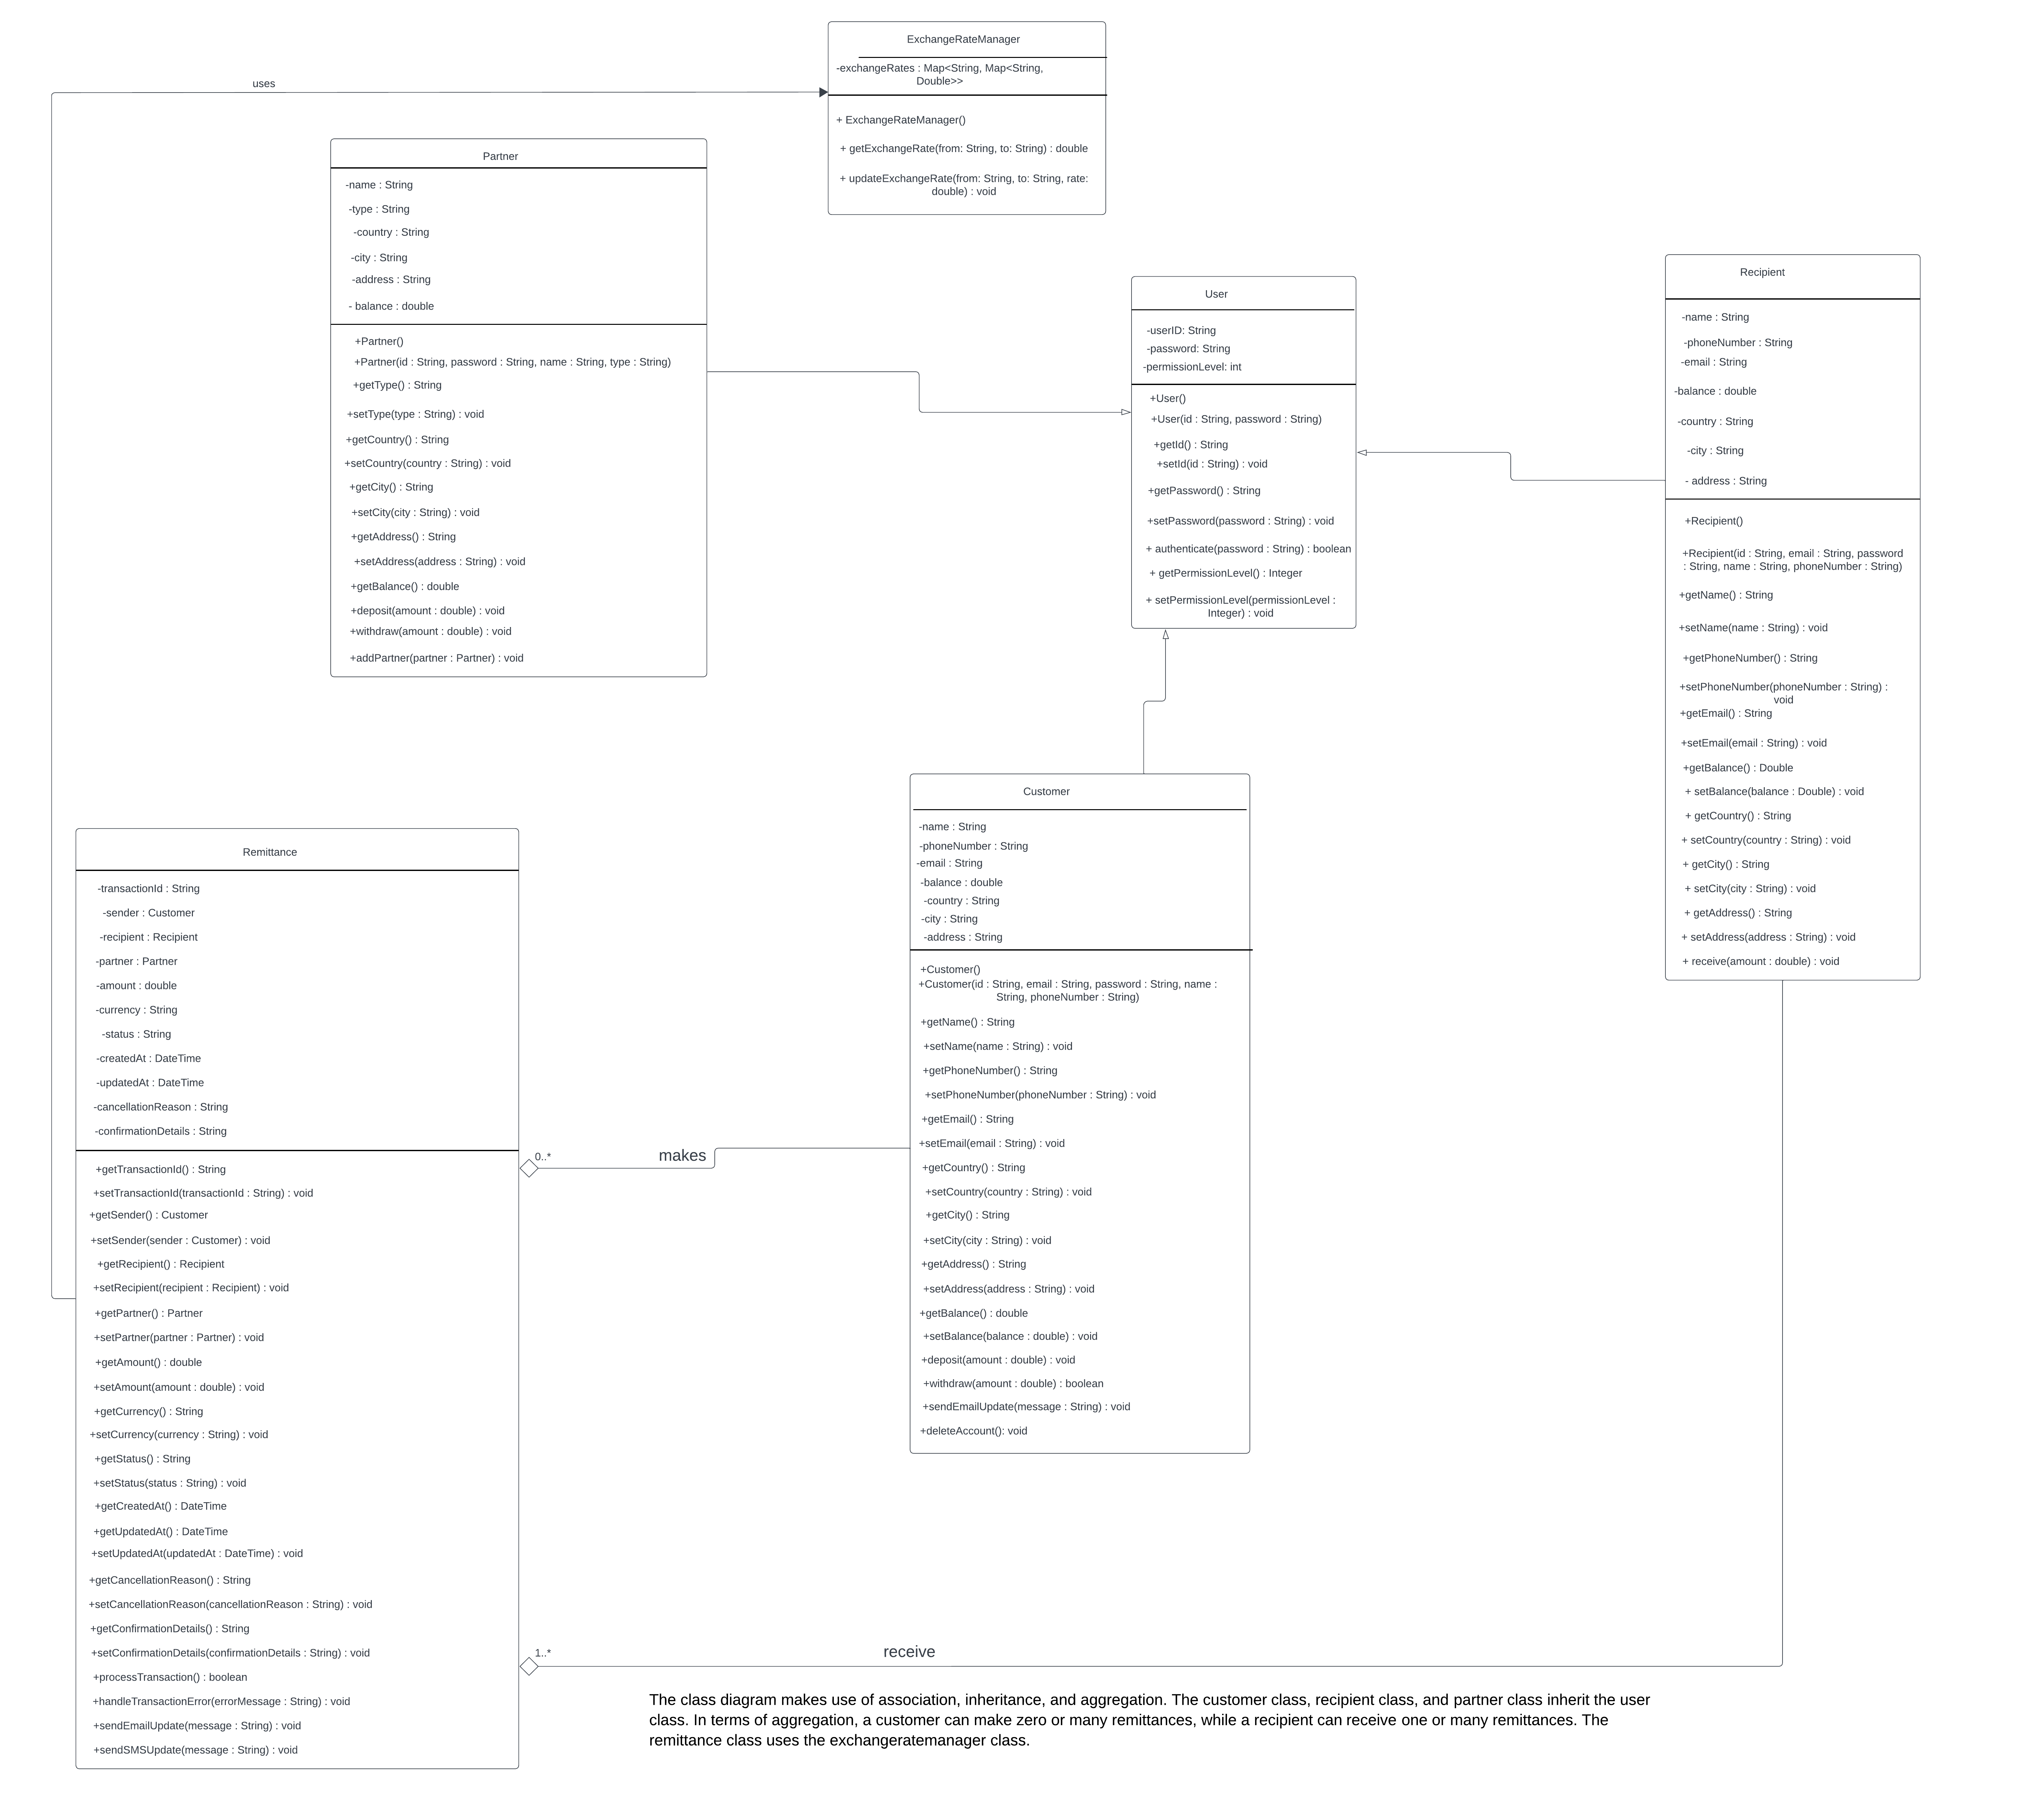
\includegraphics[width=1\linewidth]{Class Diagram.png}
    \caption{Enter Caption}
    \label{fig:enter-label}
\end{figure}
    
\end{frame}


\begin{frame}{Database Design}
These tables hold all the information needed for our business logic ensuring security, persistence and granularity of data. That includes details of the sender, recipient and also the partners that facilitate the transfer to the recipient in their home country. There is also a table for transactional data. We have placed the fact transaction table at the center of our star schema with the rest of tables serving as dimensions that augment the meaning of each transaction. This way we hope our data is structure to meet the current business needs as well as future needs such as analytical queries. For example, we should be able to track the growth rate and flow of remittances between countries or regions.

        AS for the file CRUD operations, we will create log exceptions. We limit ourselves to using a Database system for the transaction because of efficiency concerns considering the volume of transactions and real-time data processing. Indexing of data, and transactional integrity are some of of the Database system features not present in plain text files. 
    
\end{frame}


\end{document}
